% 2024 新高考Ⅰ卷 17：四棱锥 P-ABCD（PA⊥底面 ABCD）
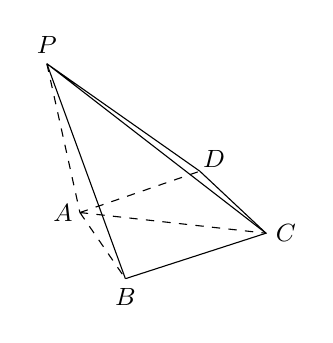
\begin{tikzpicture}[scale=1.05, font=\small]
  \coordinate (P) at (0.75,2.6);
  \coordinate (A) at (1.15,0.8);
  \coordinate (B) at (1.7,0);
  \coordinate (C) at (3.4,0.55);
  \coordinate (D) at (2.6,1.3);
  \draw (P) -- (B)  (P) -- (C)  (P) -- (D);
  \draw (B) -- (C) -- (D);
  \draw[dashed] (P) -- (A);
  \draw[dashed] (A) -- (B)  (A) -- (D)  (A) -- (C);
  \node[above] at (P) {$P$};
  \node[left, inner sep=2.5pt] at (A) {$A$};
  \node[below] at (B) {$B$};
  \node[right] at (C) {$C$};
  \node[above right, inner sep=1pt] at (D) {$D$};
\end{tikzpicture}
